\documentclass[10pt,landscape]{article}
\usepackage{multicol}
\usepackage{calc}
\usepackage{ifthen}
\usepackage[landscape]{geometry}
\usepackage{amsmath,amsthm,amsfonts,amssymb}
\usepackage{color,graphicx,overpic}
\usepackage{hyperref}


\pdfinfo{
  /Title (example.pdf)
  /Creator (TeX)
  /Producer (pdfTeX 1.40.0)
  /Author (Seamus)
  /Subject (Example)
  /Keywords (pdflatex, latex,pdftex,tex)}

% This sets page margins to .5 inch if using letter paper, and to 1cm
% if using A4 paper. (This probably isn't strictly necessary.)
% If using another size paper, use default 1cm margins.
\ifthenelse{\lengthtest { \paperwidth = 11in}}
    { \geometry{top=.5in,left=.5in,right=.5in,bottom=.5in} }
    {\ifthenelse{ \lengthtest{ \paperwidth = 297mm}}
        {\geometry{top=1cm,left=1cm,right=1cm,bottom=1cm} }
        {\geometry{top=1cm,left=1cm,right=1cm,bottom=1cm} }
    }

% Turn off header and footer
\pagestyle{empty}

% Redefine section commands to use less space
\makeatletter
\renewcommand{\section}{\@startsection{section}{1}{0mm}%
                                {-1ex plus -.5ex minus -.2ex}%
                                {0.5ex plus .2ex}%x
                                {\normalfont\large\bfseries}}
\renewcommand{\subsection}{\@startsection{subsection}{2}{0mm}%
                                {-1explus -.5ex minus -.2ex}%
                                {0.5ex plus .2ex}%
                                {\normalfont\normalsize\bfseries}}
\renewcommand{\subsubsection}{\@startsection{subsubsection}{3}{0mm}%
                                {-1ex plus -.5ex minus -.2ex}%
                                {1ex plus .2ex}%
                                {\normalfont\small\bfseries}}
\makeatother

% Define BibTeX command
\def\BibTeX{{\rm B\kern-.05em{\sc i\kern-.025em b}\kern-.08em
    T\kern-.1667em\lower.7ex\hbox{E}\kern-.125emX}}

% Don't print section numbers
\setcounter{secnumdepth}{0}


\setlength{\parindent}{0pt}
\setlength{\parskip}{0pt plus 0.5ex}

%My Environments
\newtheorem{example}[section]{Example}
% -----------------------------------------------------------------------

\begin{document}
\raggedright
\footnotesize
\begin{multicols}{3}


% multicol parameters
% These lengths are set only within the two main columns
%\setlength{\columnseprule}{0.25pt}
\setlength{\premulticols}{1pt}
\setlength{\postmulticols}{1pt}
\setlength{\multicolsep}{1pt}
\setlength{\columnsep}{2pt}

%\begin{center}
%     \Large{\underline{CS 61C}} \\
%\end{center}

\subsection{WSC}
{\bf Strong scaling} - adding more machines make algorithm faster on a given data\\
{\bf Weak Scaling} - adding more machines lets you process more data in the same amount of time \\
{\bf Data Level Parallelism} - independent	data	sets	with independent processing.\\
{\bf Big Idea} - instead of using expensive super computers use 10,000 - 100,000 cheeper servers \& networks \\
\hspace{5pt} $\cdot$ emphasize cost efficiency\\ 
\hspace{5pt} $\cdot$ attention to power: distribution \& cooling\\
\hspace{5pt} $\cdot$ (relatively) homogenous hardware/software, which is good for error handling and scaling\\ 
{\bf Quick Facts}: \\
$\cdot$ CAPEX - cost to buy equipment (buy servers)\\
$\cdot$ OPEX - cost to run equipment (electricity used)\\
$\cdot$ servers cost most \$\$\$ with replacement every 3 years\\
$\cdot$ building cooling increase PUE \\ 
$\cdot$ a lot of servers sit idle (most servers are at 10\% - 50\% max load) and waste energy \\
$\cdot$ ultimate goal is energy proportionality - \%peak load = \%peak energy\\
{\bf Power Usage Effectiveness (PUE)} = $\frac{Total Building Power}{IT Power}$\\ can never be less than 1 \\ tells us nothing about the efficiency of our computing hardware, only the relative efficiency of our IT equip vs. non IT equip.\\

\subsection{MapReduce}
{\bf Map} - slice data into shards, distribute to workers, compute sub-problem\\
map(inKey, inVal) $\rightarrow$ list(outKey, intermedVal)\\
{\bf Combiner} - compress the output of a single mapper to save on bandwidth and to distribute work more evenly \\ 
apply reduce operation distributed across map tasks, producing set of intermediate pairs\\
{\bf Reducer} - collect and combine subproblems, combining all intermediate values for a particular key to produce a set of merged output values \\
all mappers must finish before any reducer can start\\
{\bf Data Shuffle/Sort} (taken care of by framework)
merges all intermediate values with same key from mapper output to produce key value pairs of \\
(intermedKey, list[all associated values])\\ 
reduce(outKey, list(intermedVal)) $\rightarrow$ list(outVal)\\

\subsection{C Programming Language}
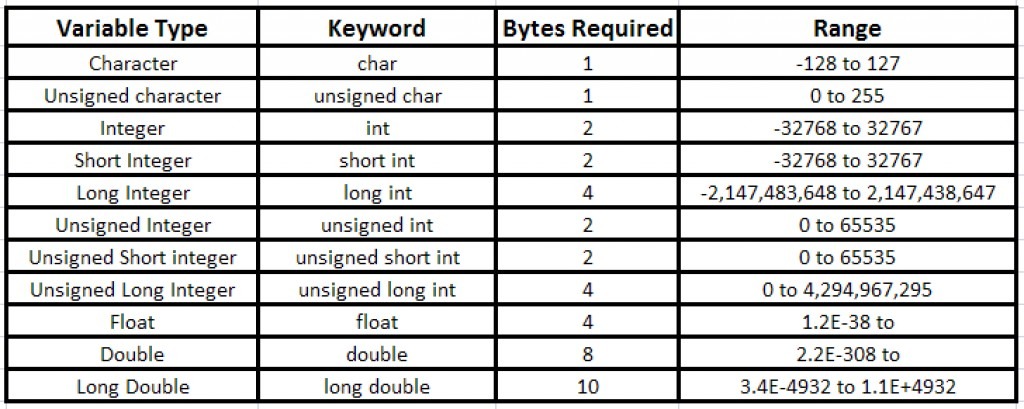
\includegraphics[scale=.2]{chart}
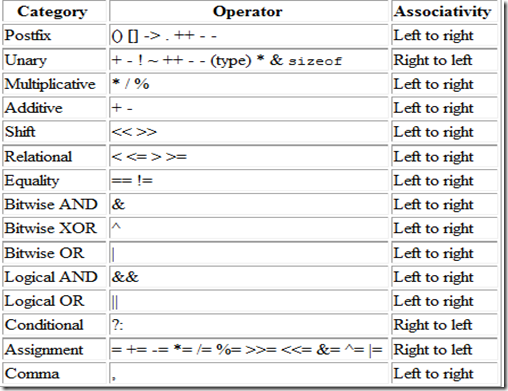
\includegraphics[scale=.5]{chart2}\\
C arrays are almost identical to pointers \\ 
array variable is a pointer to the first (0$^{th}$) element\\
arr[0] = *arr \\
arr[2] = *(arr+2)\\
must pass array \& size because array in C does not know its own length\\
arr[i] = *(arr + i)

\subsection{MIPS}
registers are 32 bits wides (this quantity is called a {\it word}), 4 bytes \\ 
memory addresses are really in bytes, not words \ \
word addresses are 4 bytes apart\\
jal - jumps to address and simultaneously saves address of following instruction in register \$ra\\
bible of MIPS - the green MIPS sheet! \\
data transfer object: constant(register used to access memory) $\rightarrow$ sum the memory address \\ 
address in a word match the address of 1 of the 4 bytes within that word\\
addresses of sequential words differ by 4 bytes \\ 
MIPS words must start at addresses that are multiples of 4\\
e.g. {\it beq \$t0, \$0, 2} $\leftarrow$ means 2 instructions, each instruction is 4 bytes (32 bits)



\subsection{C Memory Model}
{\bf $\cdot$ Stack}\\
\hspace{5pt} $\cdot$ local variables, broken into stack frames, grows down\\
{\bf $\cdot$ Heap}\\
\hspace{5pt} $\cdot$ stores data for which space was allocated with malloc(), grows upwards\\
{\bf $\cdot$ Static}\\
\hspace{5pt} $\cdot$ global, static variables, \& string literals\\
\hspace{5pt} $\cdot$ fixed size during execution\\
{\bf $\cdot$ Code}\\
\hspace{5pt} $\cdot$ contains instructions, fixed size during exec\\
 
 \subsubsection{High Level $\rightarrow$ Compiler $\rightarrow$ Assembly Language $\rightarrow$ Assembler $\rightarrow$ Binary Instructions}
\subsection{Below the Program}
\subsubsection{Operating System}
interfaces between user's application \& hardware \\
$\cdot$ handles input/output operations \\
$\cdot$ allocates memory \& storage \\
$\cdot$ provides sharing of computer among multiple applications \\

\subsubsection{Compiler}
a program that translates high level language statements into assembly language statements, symbolic representations of machine instructions
\subsubsection{Assembler}
input - assembly language code\\
output - object code\\
reads \& uses directives, replaces pseudo instructions, produces machine language, \& creates object files\\
assembler directions: \\
\hspace{5pt} $\cdot$ .text - subsequent items put in user text segment\\
\hspace{5pt} $\cdot$ .data - subsequent items put in user data segment\\
\hspace{5pt} $\cdot$ .globl sum - declares sum global and can be referenced from other files \\ 
\hspace{5pt} $\cdot$ .ascii str - store the string str in memory and null terminate it \\
\hspace{5pt} $\cdot$ .word w$_{1}$ - store a s32 bit quantity in successive memory words \\ 

\subsubsection{Object Module}
assembler or compiler translates program into machine instructions \\ 
provides information for building a complete program from the pieces:\\
\hspace{5pt} $\cdot$ header: contents of object module\\
\hspace{5pt} $\cdot$ text: translated instructions\\
\hspace{5pt} $\cdot$ static data segment: data allocated for life of program\\
\hspace{5pt} $\cdot$ relocation info: for contents that depend on absolute location of program \\
\hspace{5pt} $\cdot$ symbol table: global definitions and external references\\
\hspace{5pt} $\cdot$ debug info: for associating with source code\\

\subsubsection{Linker} 
produces executable image\\
\hspace{5pt} $\cdot$ merges segments \\ 
\hspace{5pt} $\cdot$ resolves labels \\
\hspace{5pt} $\cdot$ patches location dependent and external references\\

\subsubsection{Loader} 
\hspace{5pt} $\cdot$ reads header to determine segment sizes\\
\hspace{5pt} $\cdot$ creates virtual address space \\ 
\hspace{5pt} $\cdot$ copy text and initialized data into memory \\
\hspace{5pt} $\cdot$ sets up arguments on stack \\ 
\hspace{5pt} $\cdot$ initializes registers \hspace{5pt} $\cdot$ jumpstarts routine \\
(interpreters are sower than compiled programs, but useful for debugging)


\newpage


\subsection{Underlying Hardware}
\subsubsection{Five Components}
\hspace{5pt} $\cdot$ input: mechanism by which comp is fed info \\ 
\hspace{5pt} $\cdot$ output: mechanism by which computer conveys result of computation \\ 
\hspace{5pt} $\cdot$ memory - storage area in which programs are kept when running and area containing data necessary by program to run \\ 
\hspace{5pt} $\cdot$ data path - component of the processor that performs arithmetic operations \\ 
\hspace{5pt} $\cdot$ control - component of the processor that commands the data path, memory, \& I/O devices according to the program instructions \\

\subsection{Floating Point}
single precision: 1 sign bit (31), 8 exponent bits (30-23), 23 fraction bits (22-0)\\
FP = (-1)$^{S} \times (1+F) \times 2^{E - bias( 127)}$ \\ 
special values:\\
\hspace{5pt} $\cdot$ $\pm$ Zero: E = 0, F= 0\\
\hspace{5pt} $\cdot$  NaN: E = 255 (all 1's), F $\neq$ 0\\
\hspace{5pt} $\cdot$ $\pm \infty$ : E = 255 (all 1's), F = 0\\
\hspace{5pt} $\cdot$ Denormalized: E = 0, F $\neq$ 0\\
underflow: negative exponent is too large to fit in exponent field\\ 
overflow: exponent is too large to be represented in exponent field \\

\subsection{Performance}
throughput/bandwidth = total amount of work done in a given time \\
to maximize performance, minimize response/execution time \\ 
Performance = $\frac{1}{execution time}$\\
$\frac{performance_{x}}{performance_{y}} = \frac{execution time_{y}}{execution time_{x}} = n, \rightarrow$ x is n times faster than y\\
response time - time to complete a task \\
CPU execution time = time CPU spends computing a task not including time spent waiting for I/O\\
User CPU time - CPU time spent in the program itself \\
System CPU time - CPU time spent in the operating system performing tasks on behalf of the program \\
clock cycles - discrete time intervals determining when events take place in the hardware \\ 
clock period - time for a complete clock cycle \\ 
clock rate - inverse of the clock period \\
\subsubsection{Performance Equations}
CPU execution time = CPU clock cycles for a program $\times$ Clock Cycle time = $\frac{CPU clock cycles for a program}{clock rate (\frac{1}{clock cycle time})}$\\
CPU clock cycles = instructions for a program $\times$ average clock cycle per instruction \\
CPI (clock cycles per instruction) - average number of clock cycles per instruction for a program, an average of all instructions executed in a program. \\
CPU time = instruction count $\times$ CPU $\times$ clock cycle time = $\frac{instruction count \times CPI}{clock rate}$\\
CPI = $\frac{CPU clock cycles}{instruction count}$\\
Time = $\frac{seconds}{program} =  \frac{instructions}{program} \times \frac{clock cycles}{instruction} \times \frac{seconds}{clock cycle}$

\subsection{Cache}
AMAT (avg. mem. access time) = hit time + miss rate $\times$ miss time \\ 
local miss rate = fraction of references to one level of cache that miss, e.g. local miss rate of L2 = $\frac{L2 misses}{L1 misses}$\\
global miss rate = fraction of references that miss in all levels of a multi-level cache\\
Tag: tells us where it came from in memory. \\
Tag bits = address size - index - offset \\
Index: which row/block to look at in cache. \\
Index bits = log$_{2}(\frac{cache size}{block size})$, in other words log of the number of blocks \\
Offset: which column of cache to look at. \\
Offset bits = log$_{2}$(block size (bytes))\\
bits per row = valid bit + dirty bit (write back cache only) + data (block size) + tag \\
cache size = 2$^{offset bits + index bits}$\\
number of blocks = cache size $\div$ block size \\
tag bits = log$_{2}(\frac{memory size}{cache size})$\\
CPI$_{stall}$ = CPI$_{ideal}$ + data miss cycles + instruction miss cycles
CPI$_{stall}$ = CPI$_{ideal}$ + L1 instruction miss cycles + L1 data miss cycles


\subsection{Types of Instructions on Types of Data}
SISD: Single instruction, single data stream, e.g. Intel Pentium 4\\
MISD: Multiple instruction, single data stream, e.g. none\\
MIMD: Multiple instruction, multiple data stream, e.g. Intel Xeon e5345\\
SIMD: Single instruction, multiple data stream, e.g. SSD Instructions of x86\\
SIMD is weakest in case or switch statements, where each execution unit must perform a different operation on its data. \\

\subsubsection{Amdalh�s Law}
Maximum speedup from parallelism = $\frac{1}{((1- P) + \frac{P}{N})}$\\
P = proportion of program parallelizable 
N = number of cores\\

\subsubsection{Signed vs. Unsigned MIPS}
sra - shift right arithmetic: sign extension! right shift for signed quantities \\
srl - shift right logical: zero extension! right shift for unsigned quantities \\
sll - shift left logical: zero extension! left shift for signed \& unsigned quantities \\


\subsubsection{Recursive MIPS Example}
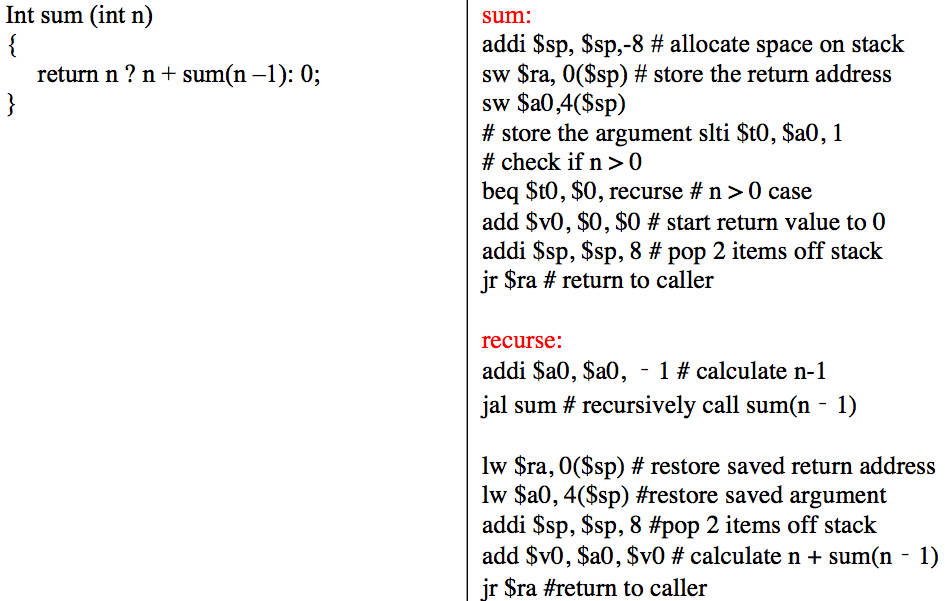
\includegraphics[scale=.25]{ex}



% You can even have references
\rule{0.3\linewidth}{0.25pt}
\scriptsize
\bibliographystyle{abstract}
\bibliography{refFile}
\end{multicols}
\end{document}